\documentclass[a4paper, 11 pt]{article}

\usepackage[latin1]{inputenc}
\usepackage[english]{babel}
\usepackage{indentfirst}
\usepackage{graphicx}
\usepackage{subfigure}
\usepackage{mathtools}
\usepackage[retainorgcmds]{IEEEtrantools}
\usepackage{multirow}
\usepackage{array}
\usepackage{mhchem}
\usepackage{booktabs}
%\usepackage{psfrag}
\usepackage[hypcap=true]{caption}
\usepackage[bookmarks=true,hyperfootnotes=false]{hyperref}
\hypersetup{
	colorlinks=true,
	linkcolor=red,
	anchorcolor=red,
	citecolor=red,
	urlcolor=red,
	%linktocpage=true
	pdftitle={THGEM characterization},
	pdfauthor={I. Ciraldo, G.A. Brischetto}
}

\newcommand{\Vind}{$\Delta V_{ind}$}
\newcommand{\Vthgem}{$\Delta V_{THGEM}$}
\newcommand{\Vdrift}{$ \Delta V_{drift}$}
\newcommand{\ibf}{$I_{bf}$}

\title{\bf {\huge FULL and ROW THGEM characterization} }
\author{Dott. D. Torresi, I. Ciraldo, G.A. Brischetto}
\date{16 Dicembre 2019}

\begin{document}

\maketitle

\section{Introduction}

In view of the upgrade of the MAGNEX Focal Plane Detector (FPD) it is necessary to test the Thick Gas Electron Multipliers (THGEMs).
This new technology will substitute the present tracker, based on proportional wires.
It guarantees to cope with rate of the order of MHz/$\mbox{mm}^2$.
The aim of these tests was to study the THGEM response varying the induction, the THGEM and the drift tensions. 
In December 2019 two prototypes of THGEM were characterized. Both prototypes are multiple THGEM composed by three layers of GEM, but they show different hole pattern for the multiplication.


%Due parole sull'obiettivo dei test, caratterizzazione delle THGEM e del prototipo, focalizzandoci sulle risposte del sistema variando le THGEM

%Descrivere i due tipi di THGEM: foto, schemi, differenze, tabella FULL THGEM vs. ROW THGEM (indicando pitch, dimensione del foro e rim, spessore totale e spessore della metallizzazione (copper plating) )


%Micro patterned gas detector


\section{Experimental setup}

In these tests, two kinds of THGEM were employed: in the first one, referred to as FULL THGEM (Figure~\ref{fig:full_thgem}), the holes are uniformly distributed over the active surface; in the second one, called ROW THGEM (Figure~\ref{fig:row_thgem}), the holes are arranged in five rows.
In the FULL THGEM there are 143 rows of holes in horizontal and in vertical direction (Figure~\ref{fig:full_thgem_holes}), giving a total of 20449 holes.
In the ROW THGEM (Figure~\ref{fig:row_thgem_holes}) for each of the five rows there are 143 holes.
The main characteristics of the two prototypes are shown in Table~\ref{tab:thgem}.
The two THGEMs have the same dimensions: 107$\times$107~$\mbox{mm}^2$.

\begin{figure}
	\centering
		\subfigure[]{\label{fig:full_thgem}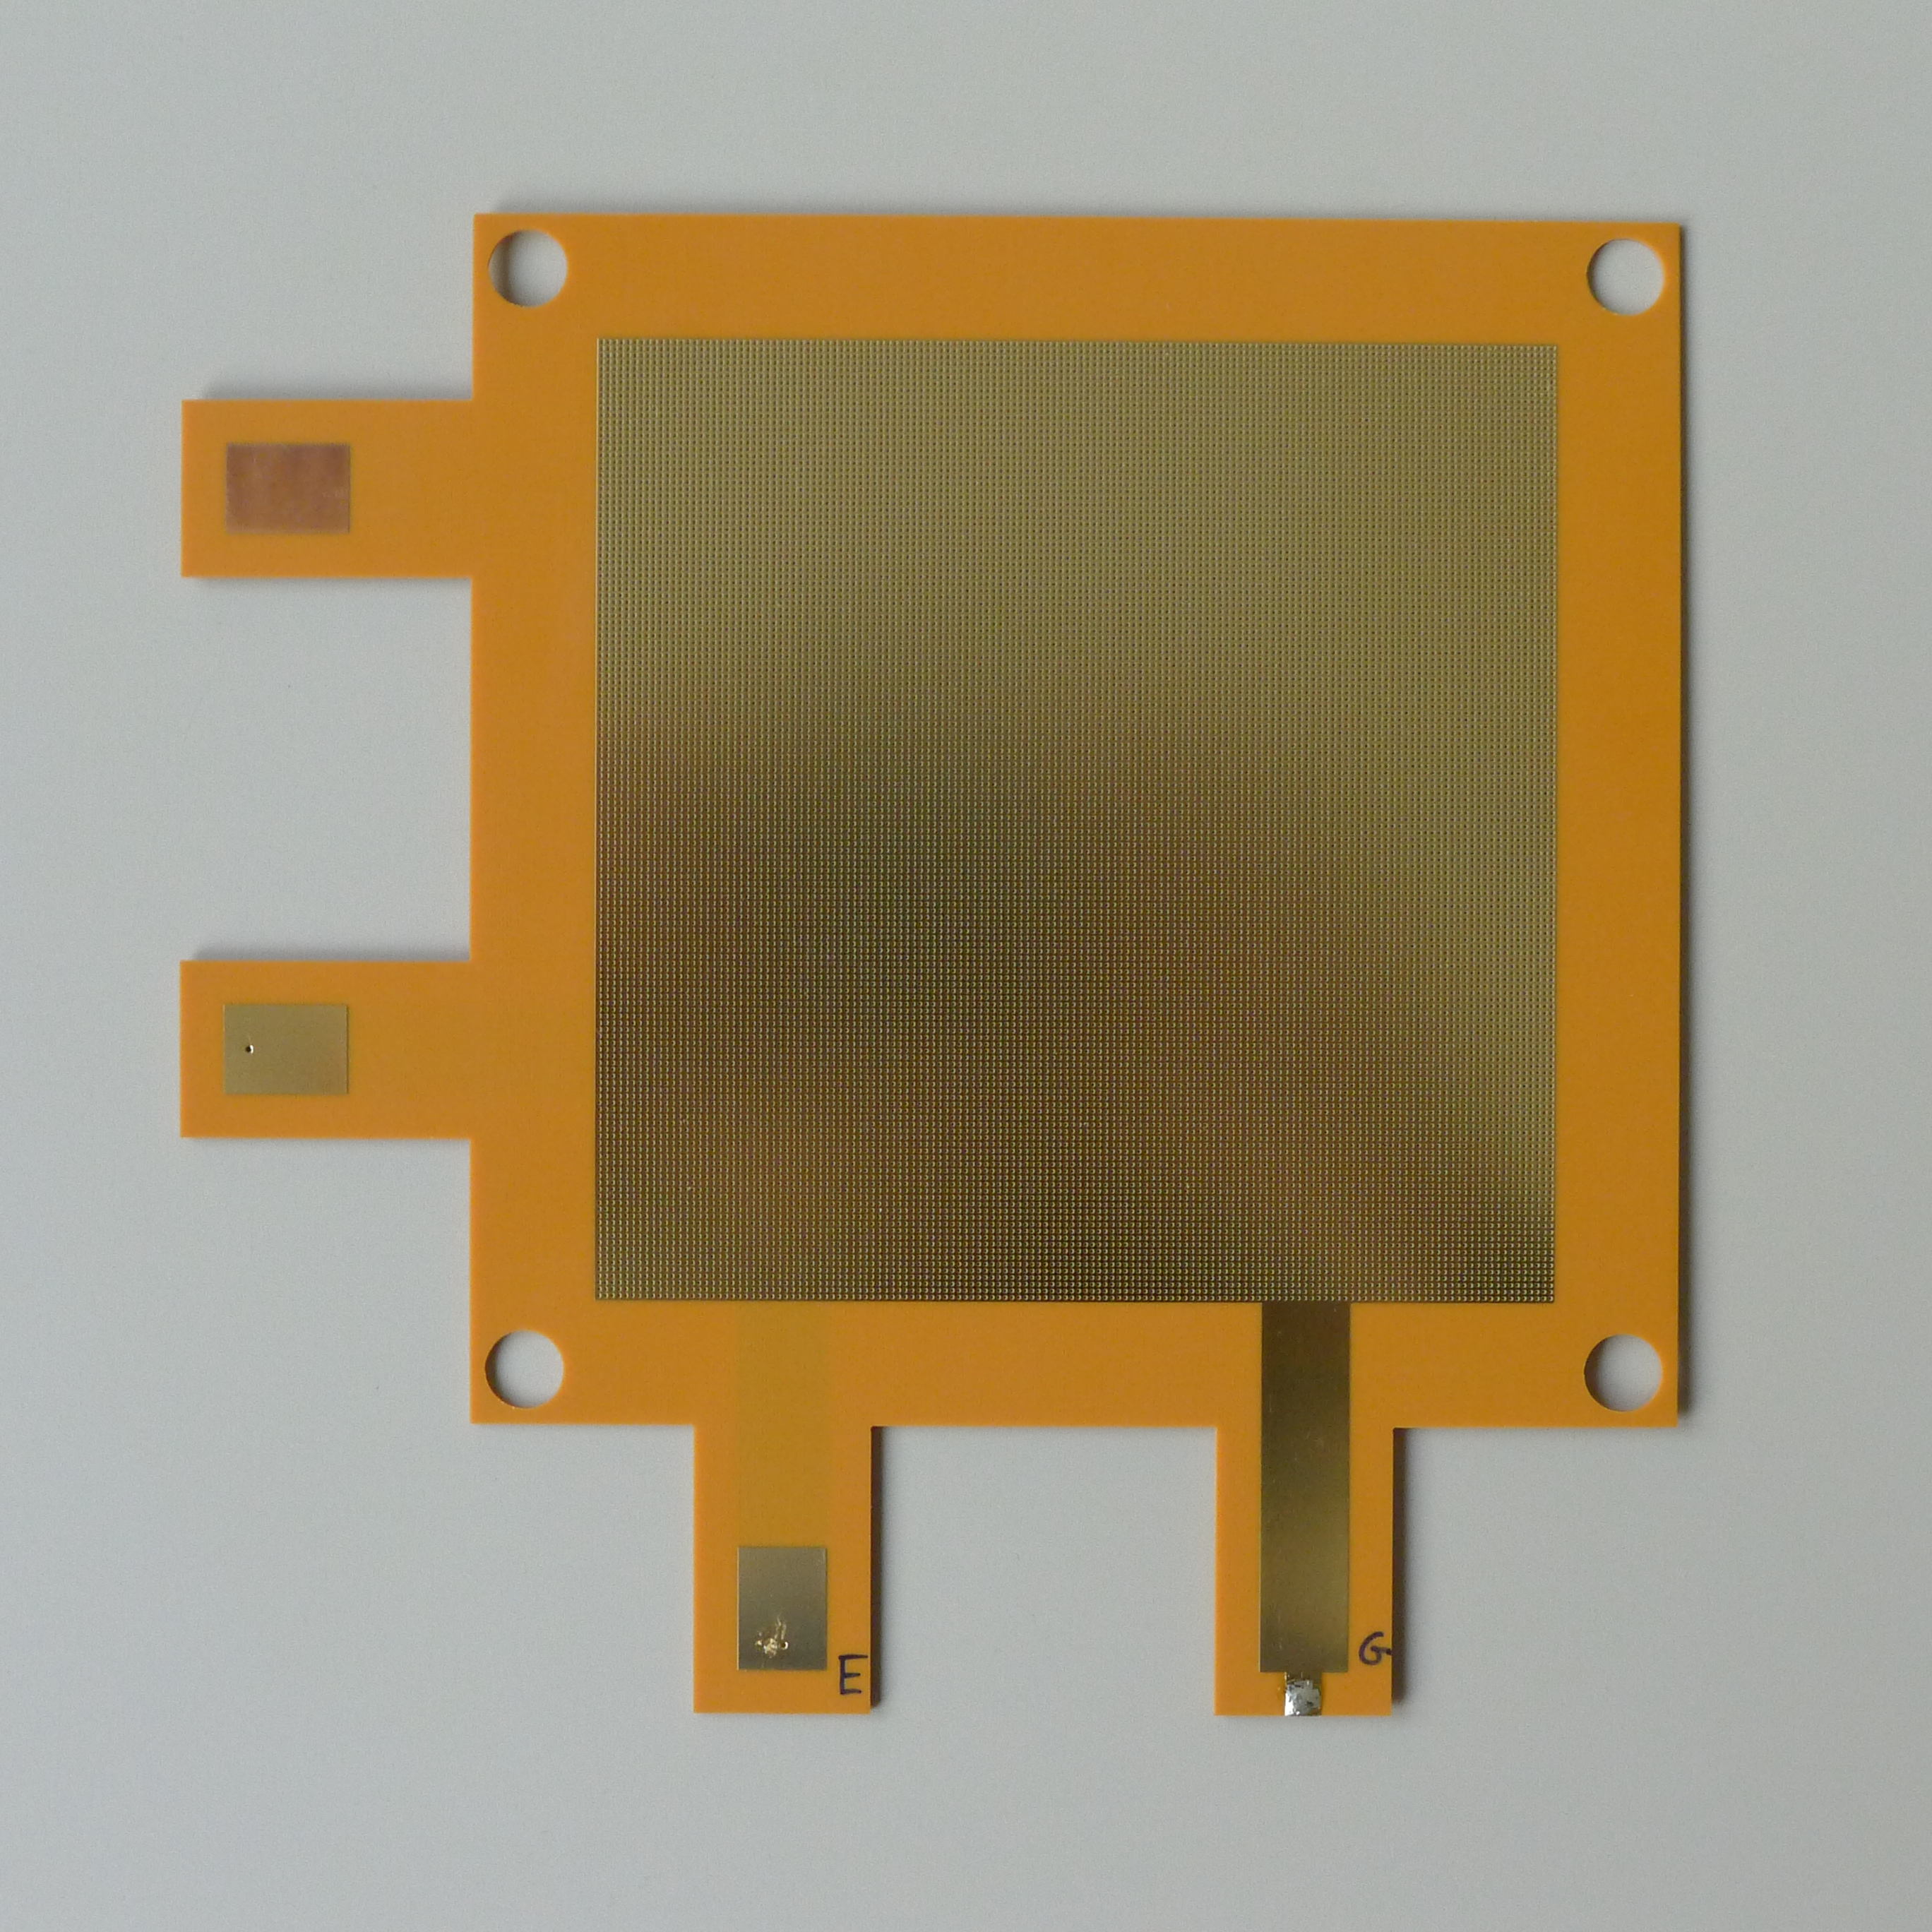
\includegraphics[width=0.45\textwidth]{Immagini/full_thgem.JPG}}
		\hspace{5pt}
		\subfigure[]{\label{fig:full_thgem_holes}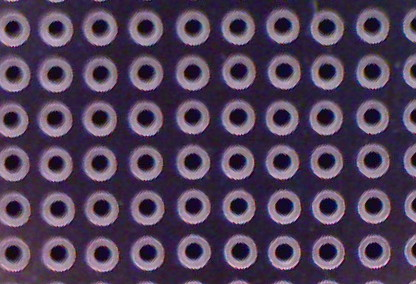
\includegraphics[width=0.45\textwidth]{Immagini/full_thgem_holes.JPG}}
	\caption{In (a) the FULL THGEM prototype, in (b) its hole pattern.}
	\label{fig:full_thgem_complessiva}		
\end{figure}

\begin{figure}
	\centering
	\subfigure[]{\label{fig:row_thgem}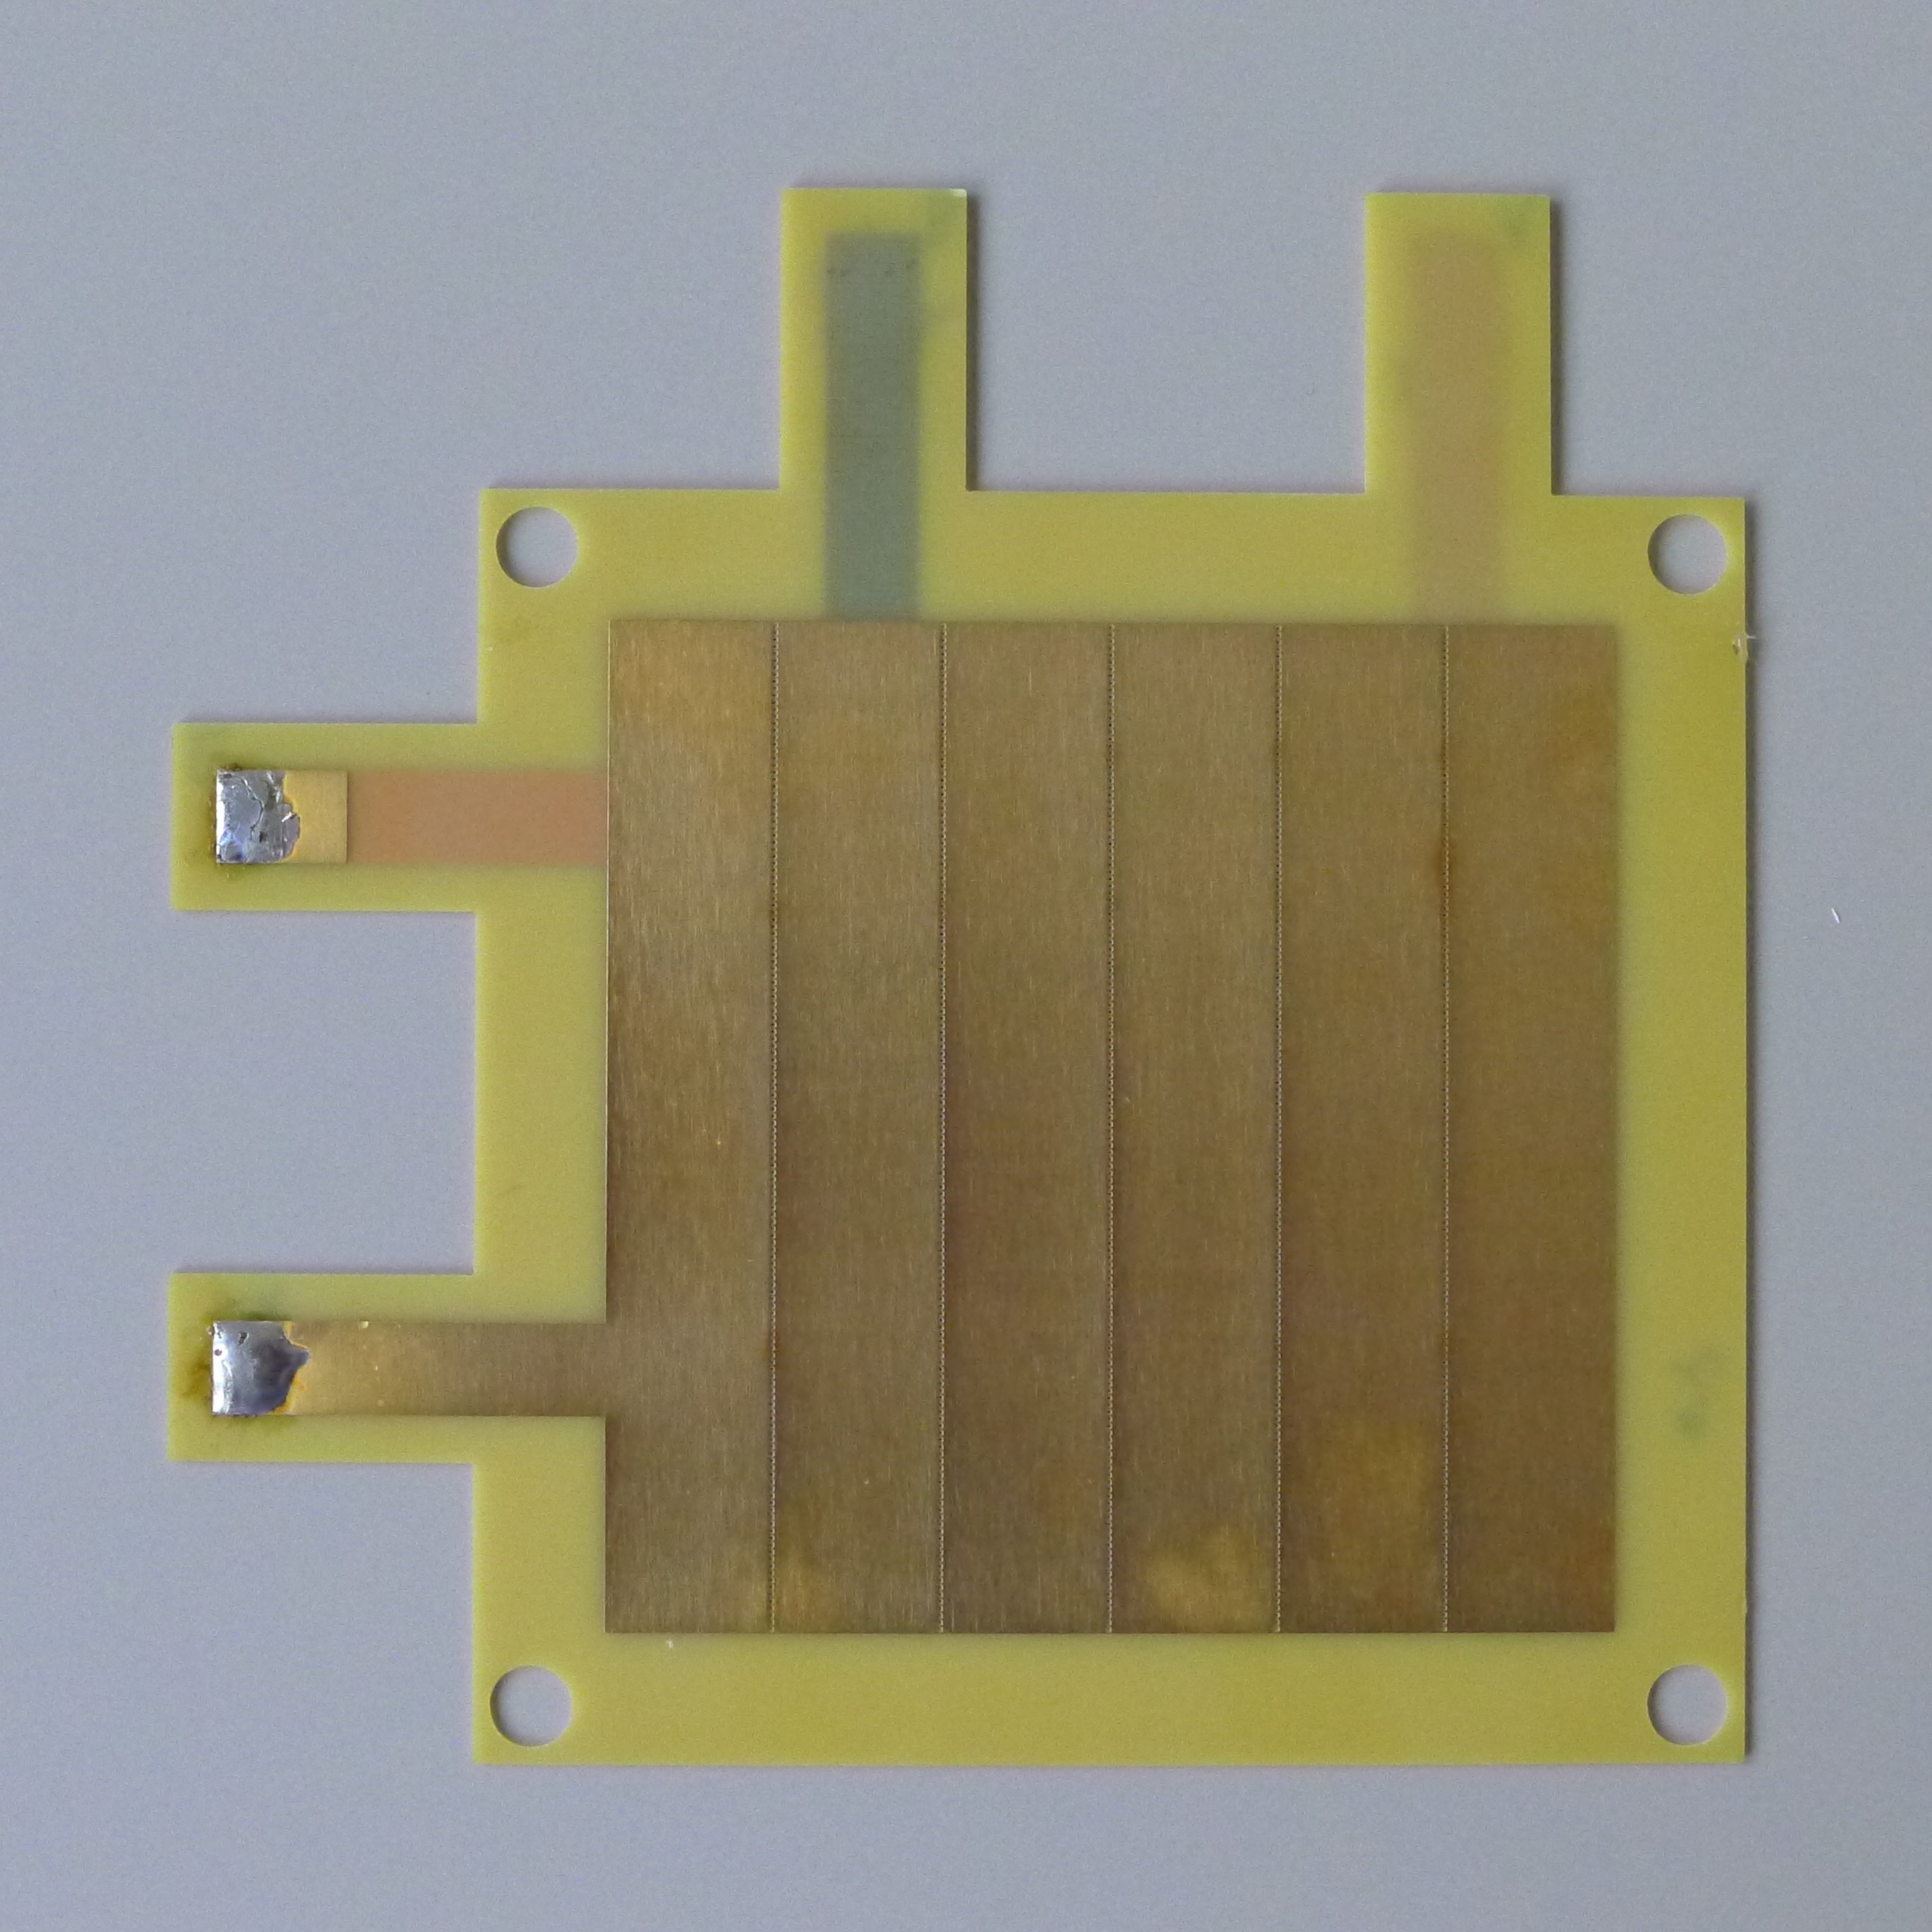
\includegraphics[width=0.45\textwidth]{Immagini/row_thgem.JPG}}
	\hspace{5pt}
	\subfigure[]{\label{fig:row_thgem_holes}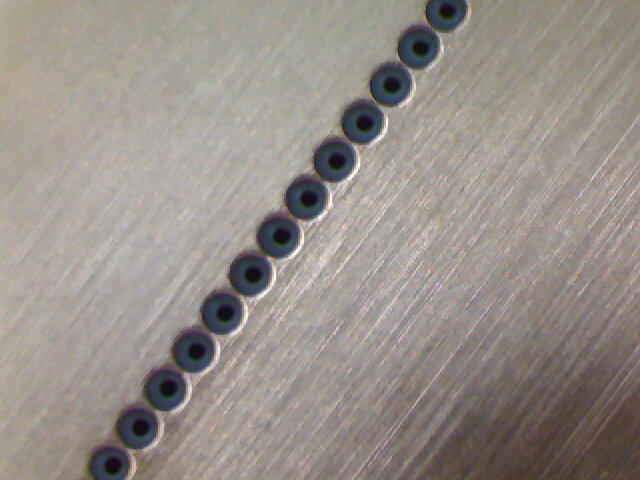
\includegraphics[width=0.45\textwidth]{Immagini/row_thgem_holes.JPG}}
	\caption{In (a) the ROW THGEM prototype, in (b) its hole pattern.}
	\label{fig:row_thgem_complessiva}		
\end{figure}

\begin{table} [b!]
	\begin{center}
		\renewcommand{\arraystretch}{1.2}
		\begin{tabular} {ccccc}
			Substrate &  Finish board   &  Hole diameter & Rim size  & Hole spacing \\
			material  &  thickness (mm) &      (mm)      &   (mm)    &   (mm)       \\
			
			\toprule[0.1em]
			%\hline
			Ceramic SD103K &  1.4 $\pm$ 0.1 & 0.30 $\pm$ 0.05 & 0.1 & 0.75 \\
			PCB 		   &  1.28 		 & 0.280		  & 0.2 & 0.75 \\
			
			\bottomrule[0.1em]
		\end{tabular}
	\end{center}
	\caption{The main characteristics of the two type of THGEM tested.} \label{tab:thgem}
\end{table}

The experimental apparatus used in the tests is composed by a gas chamber with inside the tracker prototype, an alpha source and a shutter. 
A scheme of the setup is shown in Figure~\ref{fig:schema_apparato}.
The alpha source is \ce{^{241}Am} with 55 kBq activity and 140 Hz alpha particle rate. 
The shutter is used to allow (open) or prevent (close) alpha particles from arriving to the tracker. 
To supply the required voltages a CAEN system is employed. This system can be used also for measuring Anode, THGEM and Cathode currents. The same currents were measured with better accuracy with the PICO system. PICO is a pico-amperometer and its accuracy is of the order of tenth of pA, instead the CAEN accuracy is 2 nA. Both CAEN and PICO acquisition systems measure at the same time six currents: anode, top3, bot3/top2, bot2/top1, bot1 and cathode as shown in Figure~\ref{fig:schema_canali}. Top3 current is referred to the current value of THGEM electrode in front of the anode. Bot3/top2 current is related to the current collected between the third and the second THGEM of the Triple THGEM while bot2/top1 is referred to the current collected between the first and the second THGEM. Bot1 current is related to the current value pf the THGEM electrode in front of the cathode.
The bot1 current measurement is less accurate than the other current measurements because the channel where this parameter is measured has a scope greater than the other channels.

\begin{figure}
	\centering
	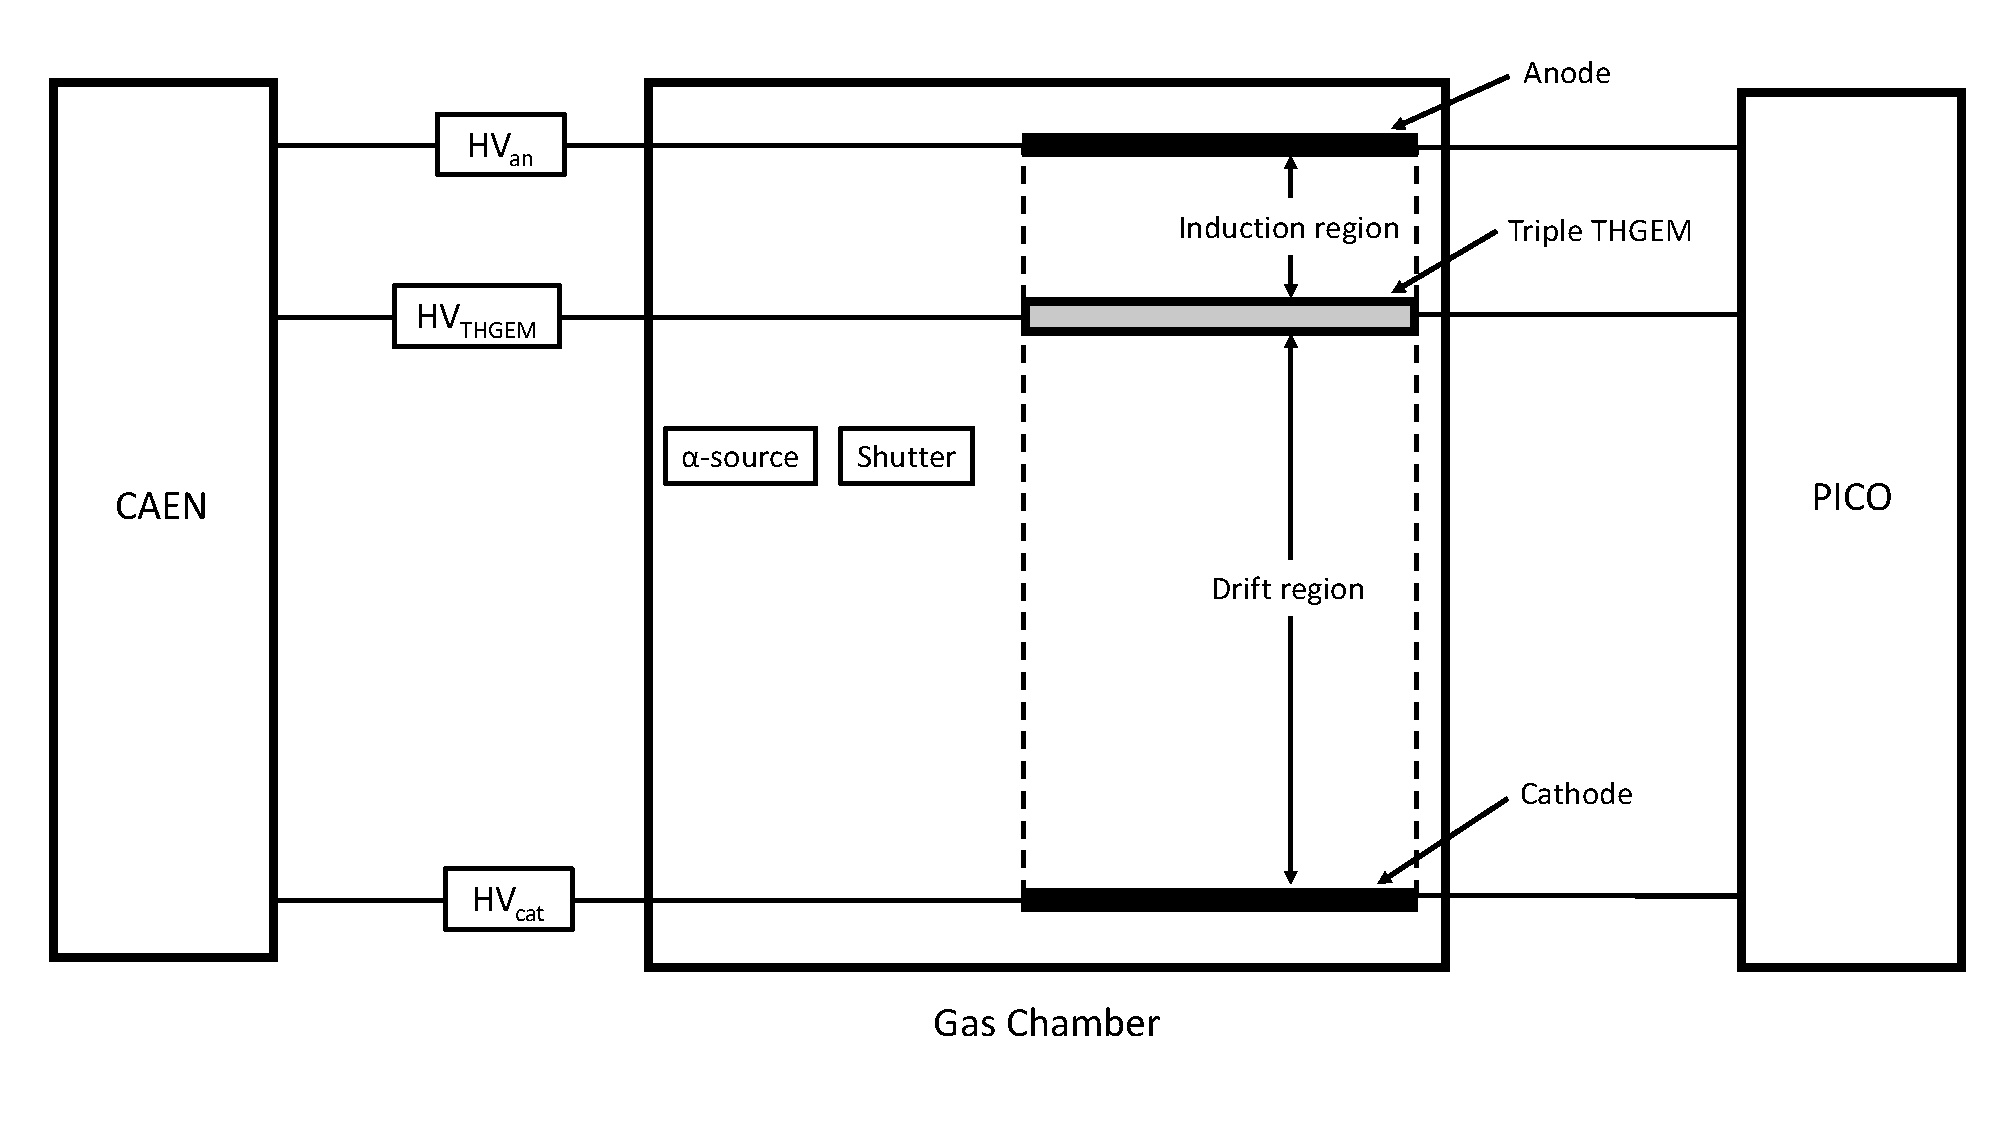
\includegraphics[width=0.9\textwidth]{Immagini/schema_apparato.pdf}
	\caption{The experimental setup.}
	\label{fig:schema_apparato}
\end{figure}

\begin{figure}
	\centering
	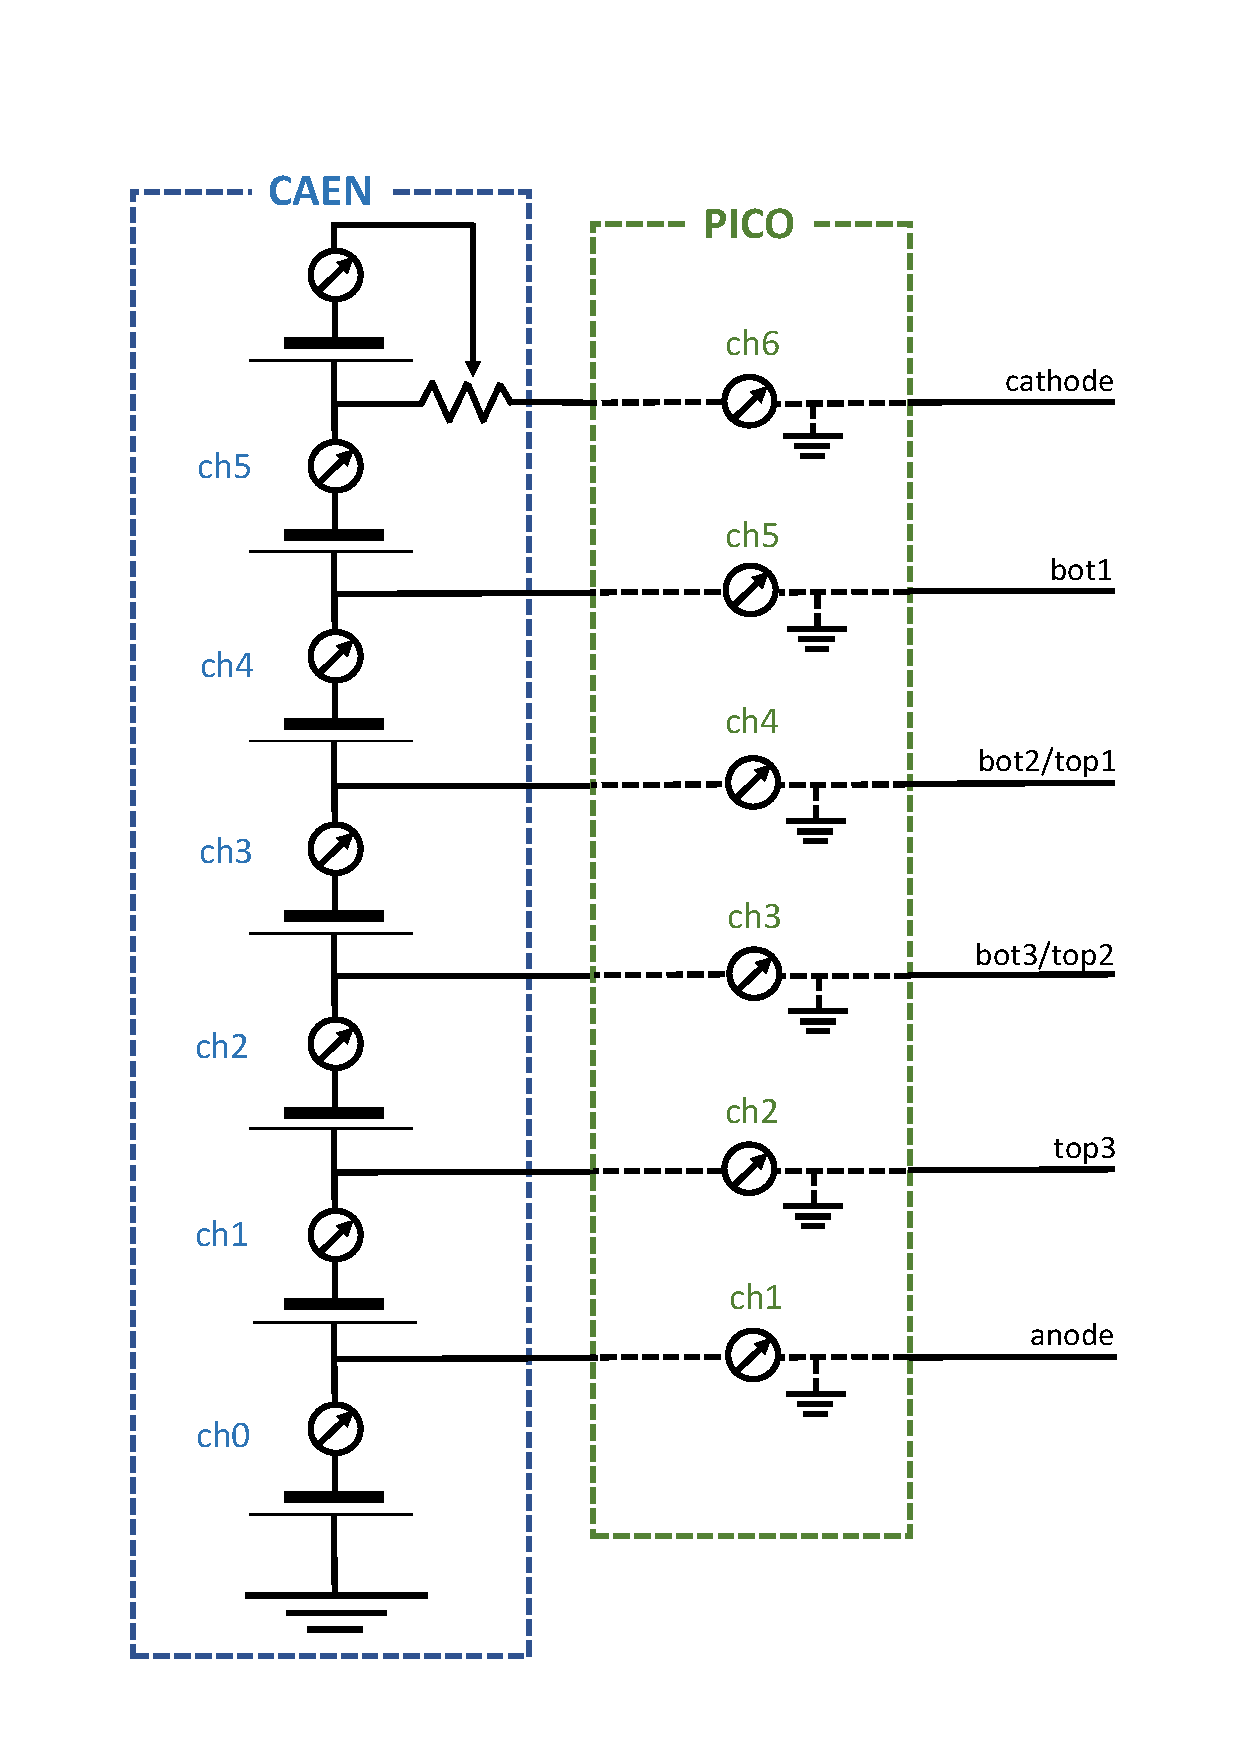
\includegraphics[width=0.8\textwidth]{Immagini/schema_canali.pdf}
	\caption{The channel scheme.}
	\label{fig:schema_canali}
\end{figure}

The gas chamber was filled with isobutane ($\mbox{C}_4\mbox{H}_{10}$) and its flow was of 145~sscm. 
The tests were performed at three different pressure: 10, 20 and 30~mbar. 



%parliamo di CAEN e PICO (non in maniera troppo approfondita)


%diagramma sui canali della lettura della corrente

inserire il plot run190 in cui si vede la misura fatta con PICO e quella con CAEN (per tutti e sei i canali!!)

%larghezza delle thgem � 107per107 mm2 e ci sono 143 file di buchi -> 20,000 buchi

%gas isobutano

%flow 145 sccm (standard cubic centimeter per minute)


range asimmetrico del bottom1, che ha minore precisione degli altri canali (farsi dire i valori da Alfonso)

\section{Method}

For a given value of pressure the induction, THGEM and drift voltages were scanned. Anode voltage was the same in each scan and it was equal to 20~V. During induction scan THGEM and drift voltages were fixed and anode, bot1, top3 and cathode currents were acquired (see Figure~\ref{fig:schema_canali}). When THGEM voltage was scanned induction and drift voltages were fixed and the same currents were acquired. Changing drift voltage value induction and THGEM voltages were fixed and the fourth currents were acquired.\\
Each run lasted 180 s acquiring anode, bot1, top3 and cathode currents. The first 60 s were dedicated to the baseline measurement with closed shutter; 90 s were employed to measure the signals with opened shutter and in the last 30 s the shutter was closed to check if the baseline level had any shifts.



%sorgente alpha e shutter, aprire e chiudere shutter, variazione di corrente

%caratteristiche sorgente (55 kBq, 241Am)

%rate di 140 Hz di particelle alpha

\section{Measurements}

%i canali 3 e 4 possono essere ignorati perch� non danno mai segnale

%spieghiamo i diversi scan (induzione, thgem e drift)

%In this section the results of 

%For the sake of clarity

\subsection{FULL THGEM}

\subsubsection{Scan on \Vind}

%The scan on \Vind aimed at studying the behaviour of 

%A preliminary study of \Vind{} variation effects on the measured currents has been done at several pressure and setting different \Vthgem{} and \Vdrift{} values.
A series of systematic measurements were conducted to study the effects of the variation of the potential difference \Vind{} on the measured currents.
These measurements have been done fixing three different pressure (P) and setting suitable values of \Vthgem{} and \Vdrift.
A summary scheme of the adopted configurations is shown in Table~\ref{tab:FULLTHGEM_vind}.
\begin{table} [b!]
	\begin{center}
		\renewcommand{\arraystretch}{1.2}
		\begin{tabular} {ccccc}
			P (mbar) & & \Vthgem{} (V) & & \Vdrift{} (V)\\
			\toprule[0.1em]
			%\hline
			30	& &	220	& &	1000 \\
			30	& &	200	& &	1000 \\
			30	& &	230	& &	1000 \\
			20	& &	200	& & 1000 \\
			11	& & 170	& & 600 \\
			
			\bottomrule[0.1em]
		\end{tabular}
	\end{center}
	\caption{The values of pressure (P), \Vthgem{} and \Vdrift{} adopted for the study on \Vind.} \label{tab:FULLTHGEM_vind}
\end{table}
%\begin{table} [b!]
%	\begin{center}
%		\renewcommand{\arraystretch}{1.2}
%		\begin{tabular} {ccccccc}
%			P (mbar) & & \Vthgem{} (V) & & \Vdrift{} (V) & & optimal \Vind{} (V) \\
%			\toprule[0.1em]
%			%\hline
%			30	& &	220	& &	1000 & & 120 \\
%			30	& &	200	& &	1000 & &  \\
%			30	& &	230	& &	1000 & & \\
%			20	& &	200	& & 1000 & & \\
%			11	& & 170	& & 600  & &\\
%			
%			\bottomrule[0.1em]
%		\end{tabular}
%	\end{center}
%	\caption{The values of pressure (P), \Vthgem{} and \Vdrift{} adopted for the study on \Vind.} \label{tab:FULLTHGEM_vind}
%\end{table}
The \Vind{} scans have been carried out starting from 0~V and increasing the voltage by 10 or 20~V per run, until the discharge value is reached (typically at more than 200~V).

The result of the scan at 30~mbar and with \Vthgem{}~=~220~V is shown in Figure~\ref{fig:induction_FULLTHGEM_30mbar}: by raising the value of \Vind{}, the anodic current (blue line) increases, while the top3 current (yellow line) approaches to zero.
\begin{figure}[htb]
	\centering
	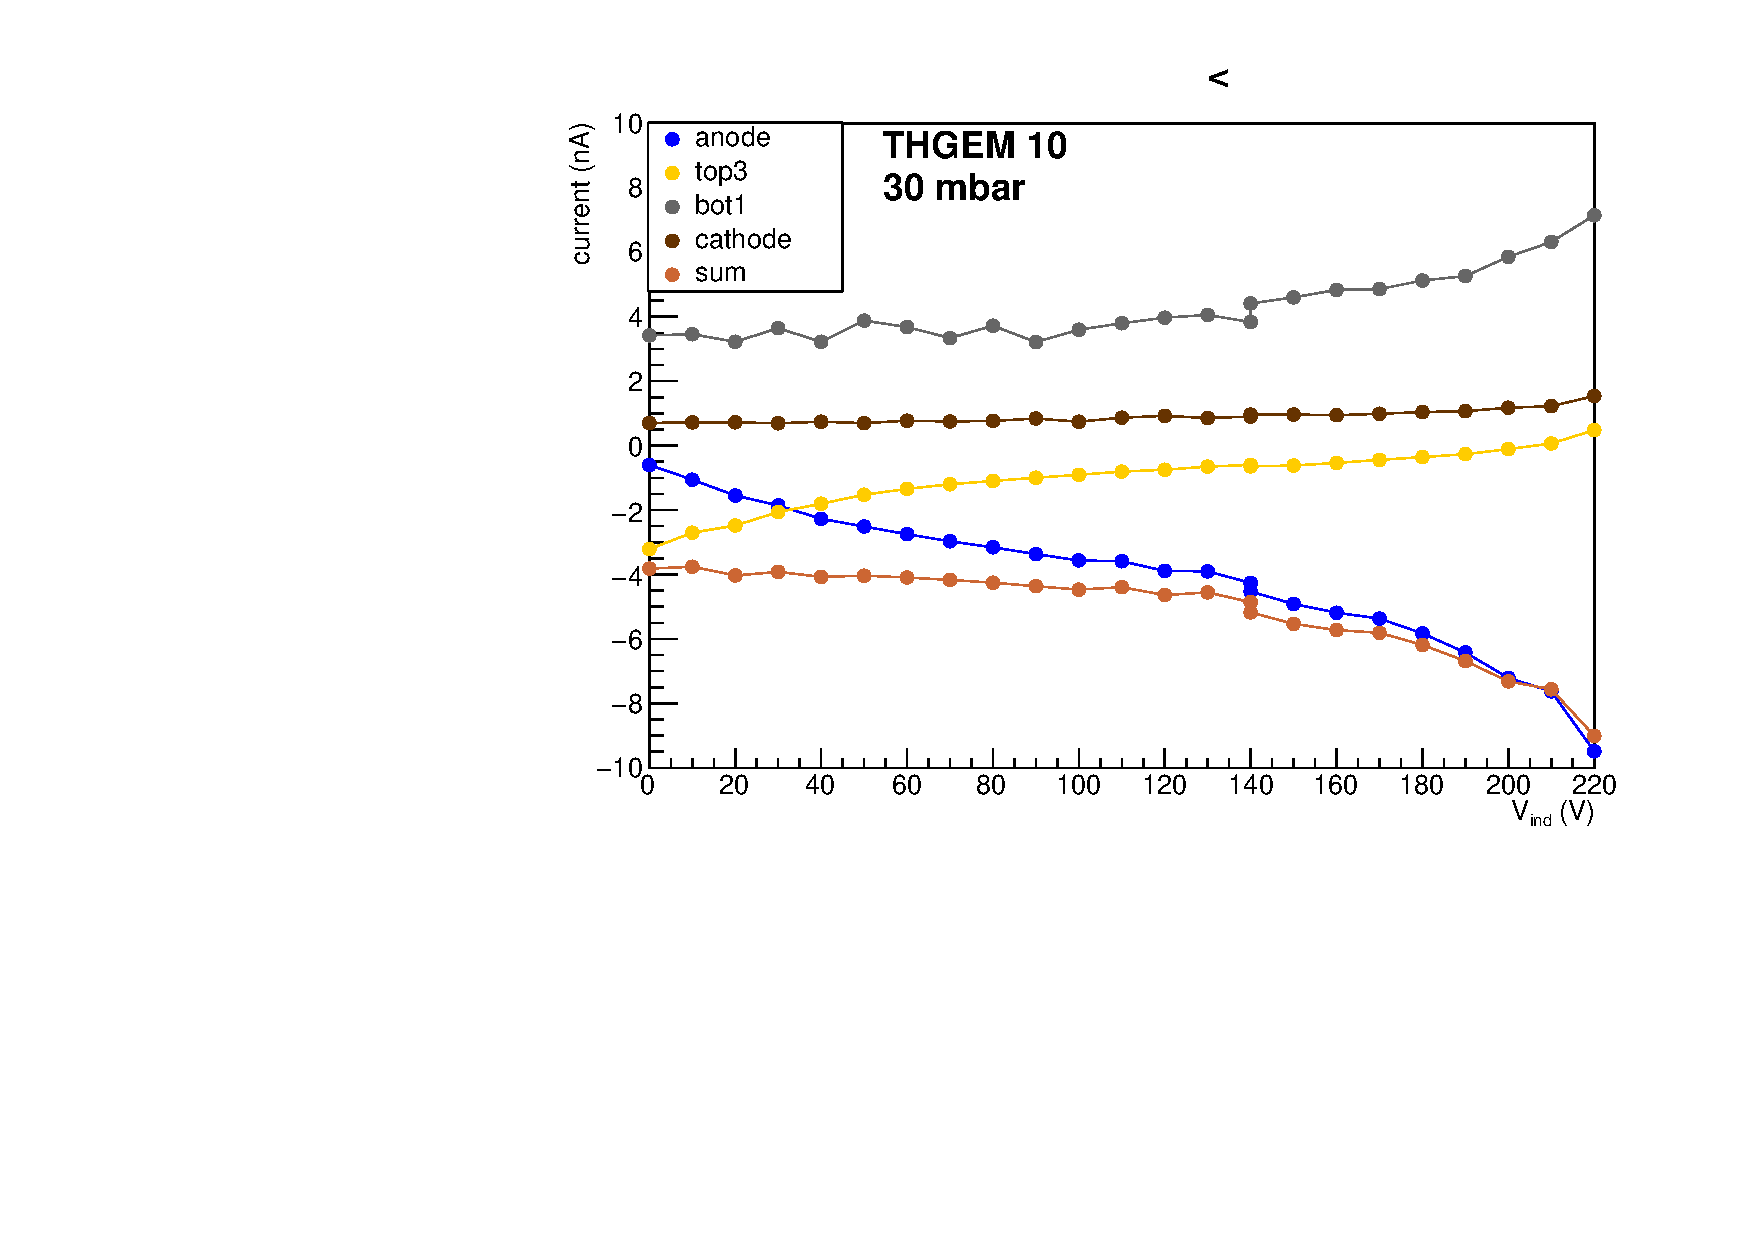
\includegraphics[width=\textwidth]{Immagini/inductionScan_THGEM10_30mbar.pdf}
	\caption{Currents measured during the scan on the voltage \Vind{} across the induction region at 30~mbar and with \Vthgem{}~=~220~V.}
	\label{fig:induction_FULLTHGEM_30mbar}
\end{figure}
Up to 140~V, their change is such that their sum (orange line) is constant.
% but their change is such that their sum (orange line) is constant.
%Up to 140~V, when \Vind{} increases, the anodic current (blue line) goes up, the top3 current (yellow line) approaches to zero, and their sum (orange line) is constant.
This means that the stronger is the electric field in the induction region, the greater is the fraction of secondary electrons collected at the anode.
%Up to 140~V, the sum of anode and top3 currents (orange line) is constant, so the 
%The total number of secondary electrons, 
%The sum of anode and top3 currents is constant 
%; in particular, for \Vind{} greater than about 30~V most electrons
%This means that when the electric field in the induction region is weak, most of the electrons produced by multiplication are collected at the top3 electrode and only a few reaches the anode.
For \Vind{} greater than 140~V, the anode and top3 currents sum increases: this behaviour can be explained considering that, when the voltage is high enough, the multiplication region extends out of the THGEM holes, occupying a section of the induction region.
The concomitant increase of the bot3 current may confirm this hypothesis.
For \Vind{} equal to 220~V, the top3 current becomes positive, so that some ions are collected at the top3 electrode.
For these values of pressure, \Vthgem{} and \Vdrift, a plateau is reached between 110 and 130~V, where the field pushes almost all the electrons from the avalanche to the anode.
In these conditions, the optimal value of \Vind{} is 120~V.


Keeping the pressure at 30~mbar, other two measurements on \Vind~{} were conducted with \Vthgem{} equal to 200 or 230~V.
The results of these measurements are shown, respectively, in Figure~\ref{fig:induction_FULLTHGEM_30mbar_other_VTHGEM_a} and ~\ref{fig:induction_FULLTHGEM_30mbar_other_VTHGEM_b}.
\begin{figure}[!htb]
	\centering
	\subfigure[]{ \label{fig:induction_FULLTHGEM_30mbar_other_VTHGEM_a} 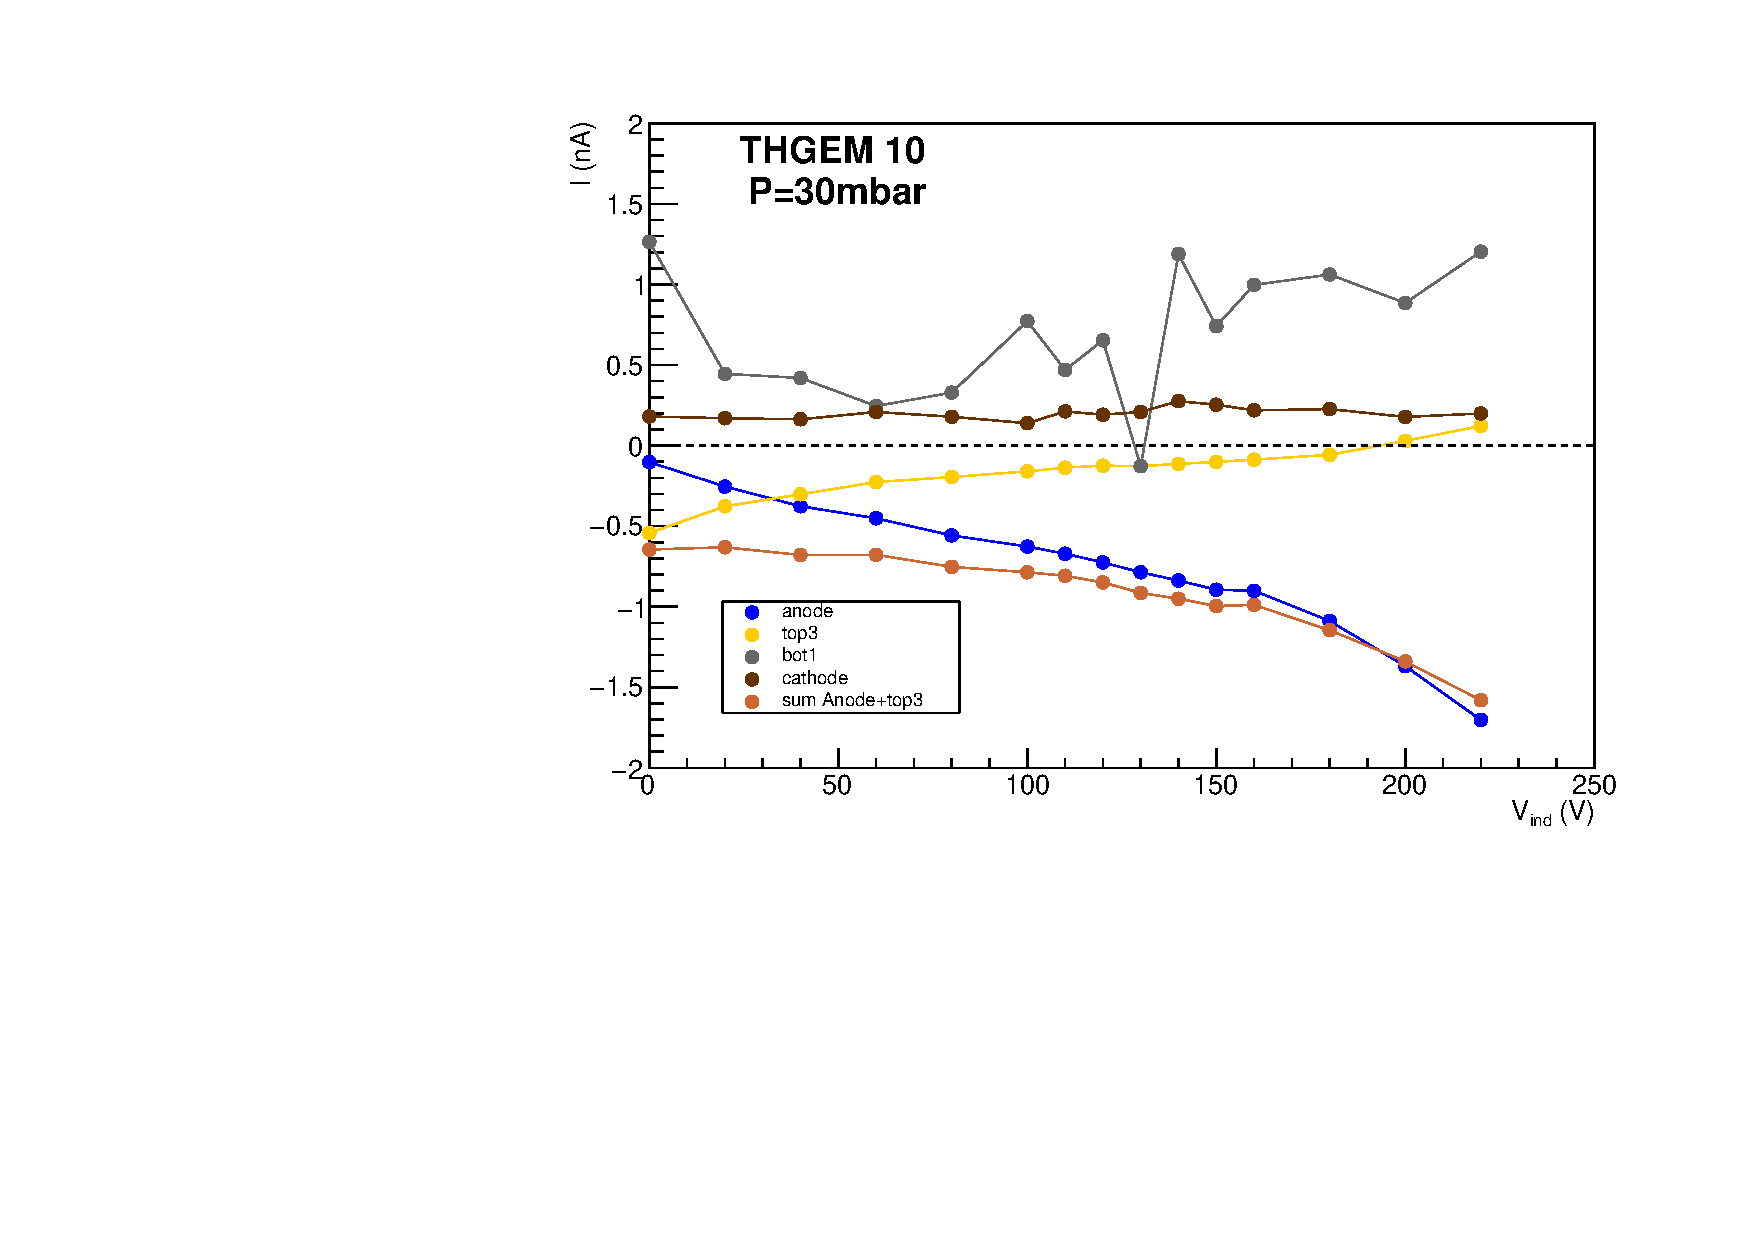
\includegraphics[width=0.96\textwidth]{Immagini/inductionScan_THGEM10_30mbar_bis.pdf}}
	\subfigure[]{ 	\label{fig:induction_FULLTHGEM_30mbar_other_VTHGEM_b} 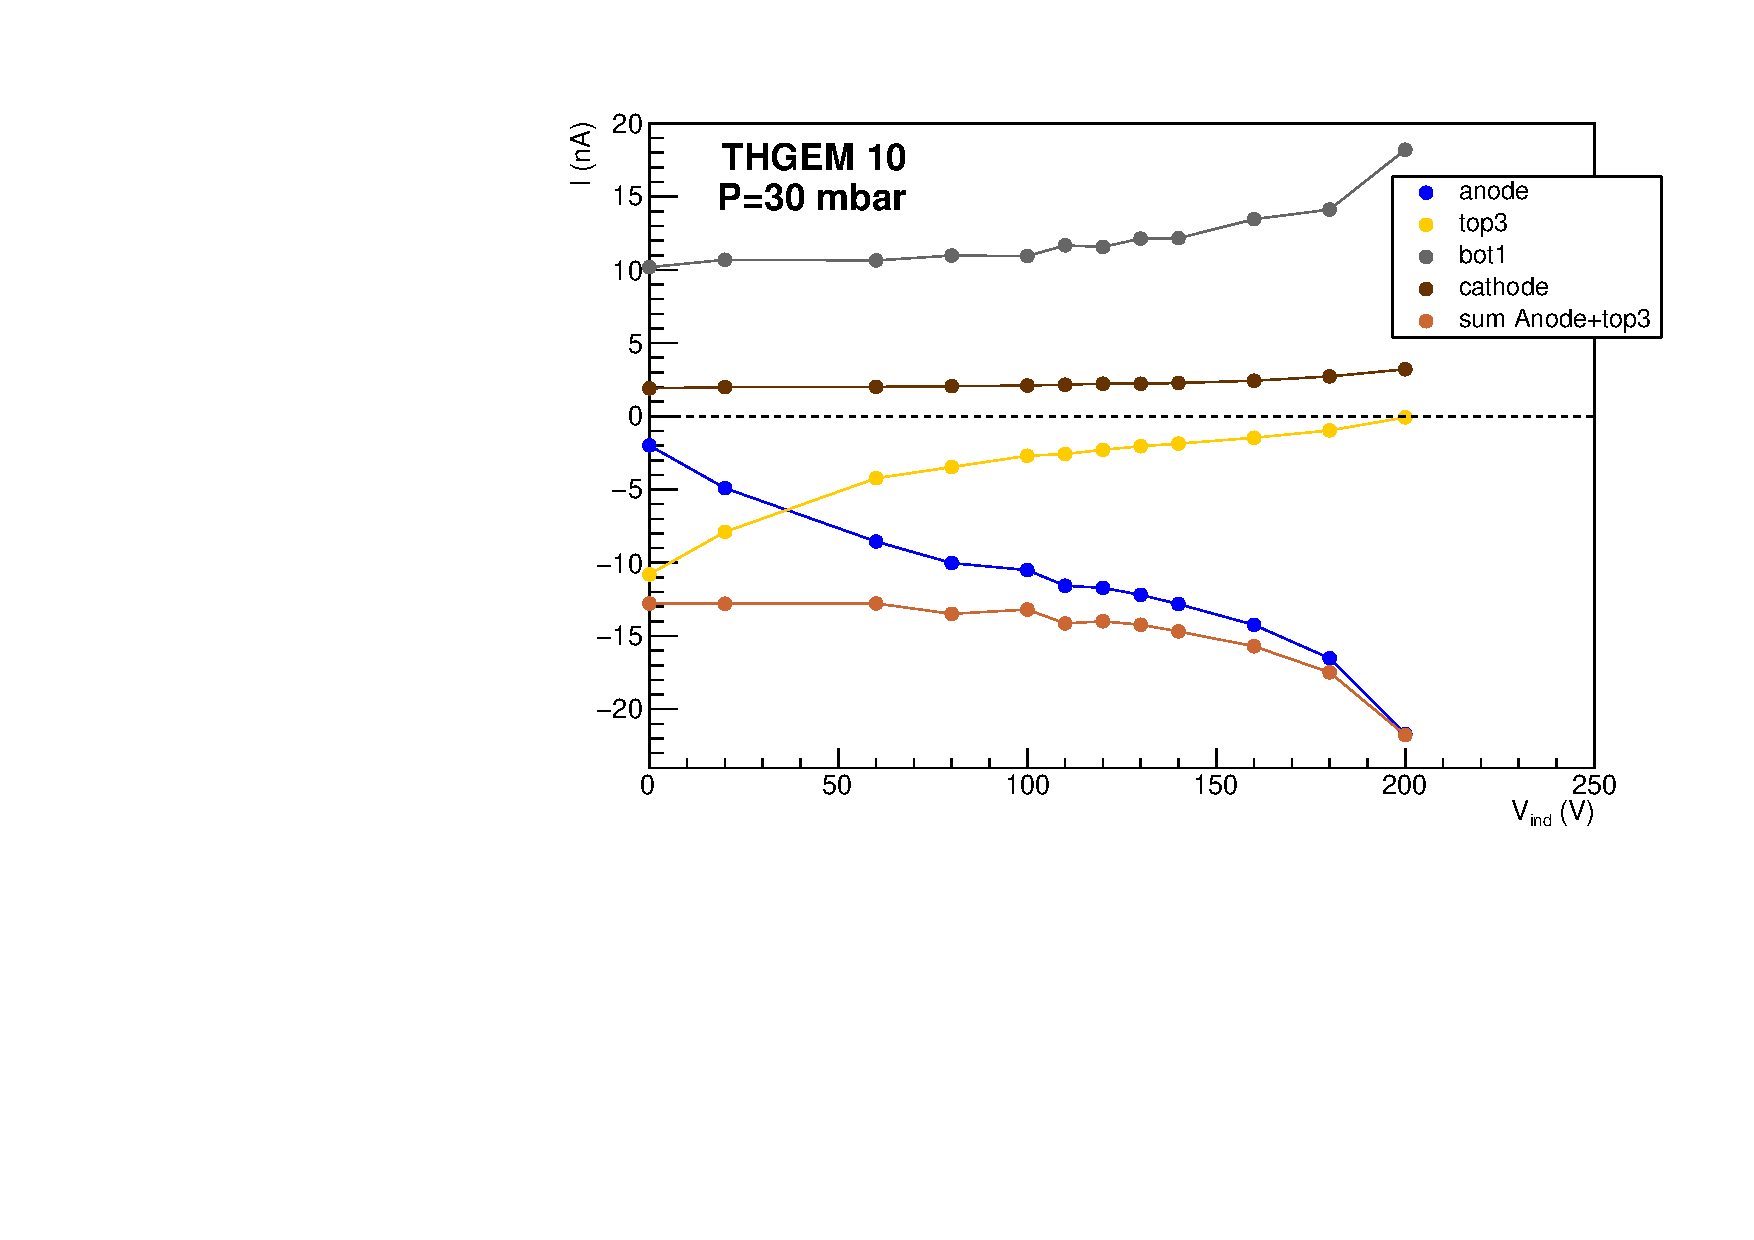
\includegraphics[width=0.96\textwidth]{Immagini/inductionScan_THGEM10_30mbar_tris.pdf}}
	\caption{Currents measured during the scan on the voltage \Vind{} across the induction region at 30~mbar: in (a) for \Vthgem~=~200~V, in (b) for \Vthgem~=~230~V.}
	\label{fig:induction_FULLTHGEM_30mbar_other_VTHGEM}
\end{figure}
The comparison between these two figures makes apparent that the magnitude of the measured currents increases with increasing \Vthgem, because the multiplication factor goes up.
Most considerations made in the case with \Vthgem~=~220~V are also valid for these two measurements, except that the plateau region is less evident or absent.
For \Vthgem~=~200~V the bot1 current fluctuations are due to the lower accuracy of the corresponding PICO channel.
\textcolor{red}{Mancano i risultati con le altre pressioni}

%Also in these two measurements, when \Vind{} increases, the anodic current increases, while the top3 current decreases. The crossing point of these two currents is still at around 32~V. After a certain value the sum of the anode and top3 current varies rapidly.

%The effects seen for \Vthgem~=~220~V appear as well in these two cases.
%The magnitude of the measured currents increases with increasing \Vthgem, because
%For \Vthgem~=~200~V the magnitude of the measured currents is lower than in the previous case, while for \Vthgem~=~230~V it is 

%as expected, increasing \Vind{} the fraction of electrons collected at the anode
%this plot displays some of the most important features



%\subsubsection*{Scan on induction voltage at 30 mbar}
%To find the optimal value for the induction voltage, a scan on this parameter has been done. The measured currents obtained for a pressure of 30~mbar and for \Vthgem~=~220~V and \Vdrift~=~1000~V are shown in Figure~\ref{fig:induction_FULLTHGEM_30mbar}. In each plot, bot2/top1 and bot3/top2 currents are not shown because their values do not change during the measurement. In Figure~\ref{fig:induction_FULLTHGEM_30mbar} is shown the sum of the anode and top3 currents. This curve has a plateau zone in the range 110$\div$130~V, so the optimal value for the \Vind is 120~V. The induction scan was repeated with \Vthgem~=~200~V and \Vthgem~=~230~V, but there was no visible plateau. In each induction scan, when the set voltage exceeds a certain value (different in the three cases), the sum of anode and top3 currents increases. This behaviour can be explained because the multiplication region extends out of the hole of the THGEM. The electric field gives a further multiplication and some ions reach the THGEM.

\subsubsection{Scan on \Vthgem}

In order to study the multiplication factor in different conditions, a series of measurements was conducted varying the voltage \Vthgem, while pressure, \Vind{} and \Vdrift{} were set to fixed values.
The variation range of \Vthgem{} was determined in this way: the lower extreme is the minimum value at which a variation of the measured currents is visible, while the higher extreme is the discharge value.
Clearly, the range depends on the selected pressure, so that for P~=~30 mbar it was from 180 to 235~V, for P~=~20~mbar it was from 150 to 215~V, and for P~=~11~mbar it was from 130 to 210~V.
The increments were ranging from 5 to 10~V.
The chosen values of pressure, \Vind{} and \Vdrift{} are shown in Table~\ref{tab:FULLTHGEM_vthgem}.

\begin{table} [!t]
	\begin{center}
		\renewcommand{\arraystretch}{1.2}
		\begin{tabular} {ccccc}
			P (mbar) & & \Vind{} (V) & & \Vdrift{} (V)\\
			\toprule[0.1em]
			%\hline
			30	& &	120	& &	1000 \\
			20	& &	100	& & 1000 \\
			11	& & 70	& & 600 \\
			
			\bottomrule[0.1em]
		\end{tabular}
	\end{center}
	\caption{The values of pressure, \Vind{} and \Vdrift{} adopted for the study on \Vthgem.} \label{tab:FULLTHGEM_vthgem}
\end{table}

Figure~\ref{fig:thgem_FULLTHGEM_30mbar} displays the result of the measurement at 30~mbar.
As \Vthgem{} increases, the currents show an exponential growth, typical of gas detectors in avalanche regime.
In these conditions, the optimal value of \Vthgem is 220~V, because it gives currents 
\begin{figure}[htb]
	\centering
	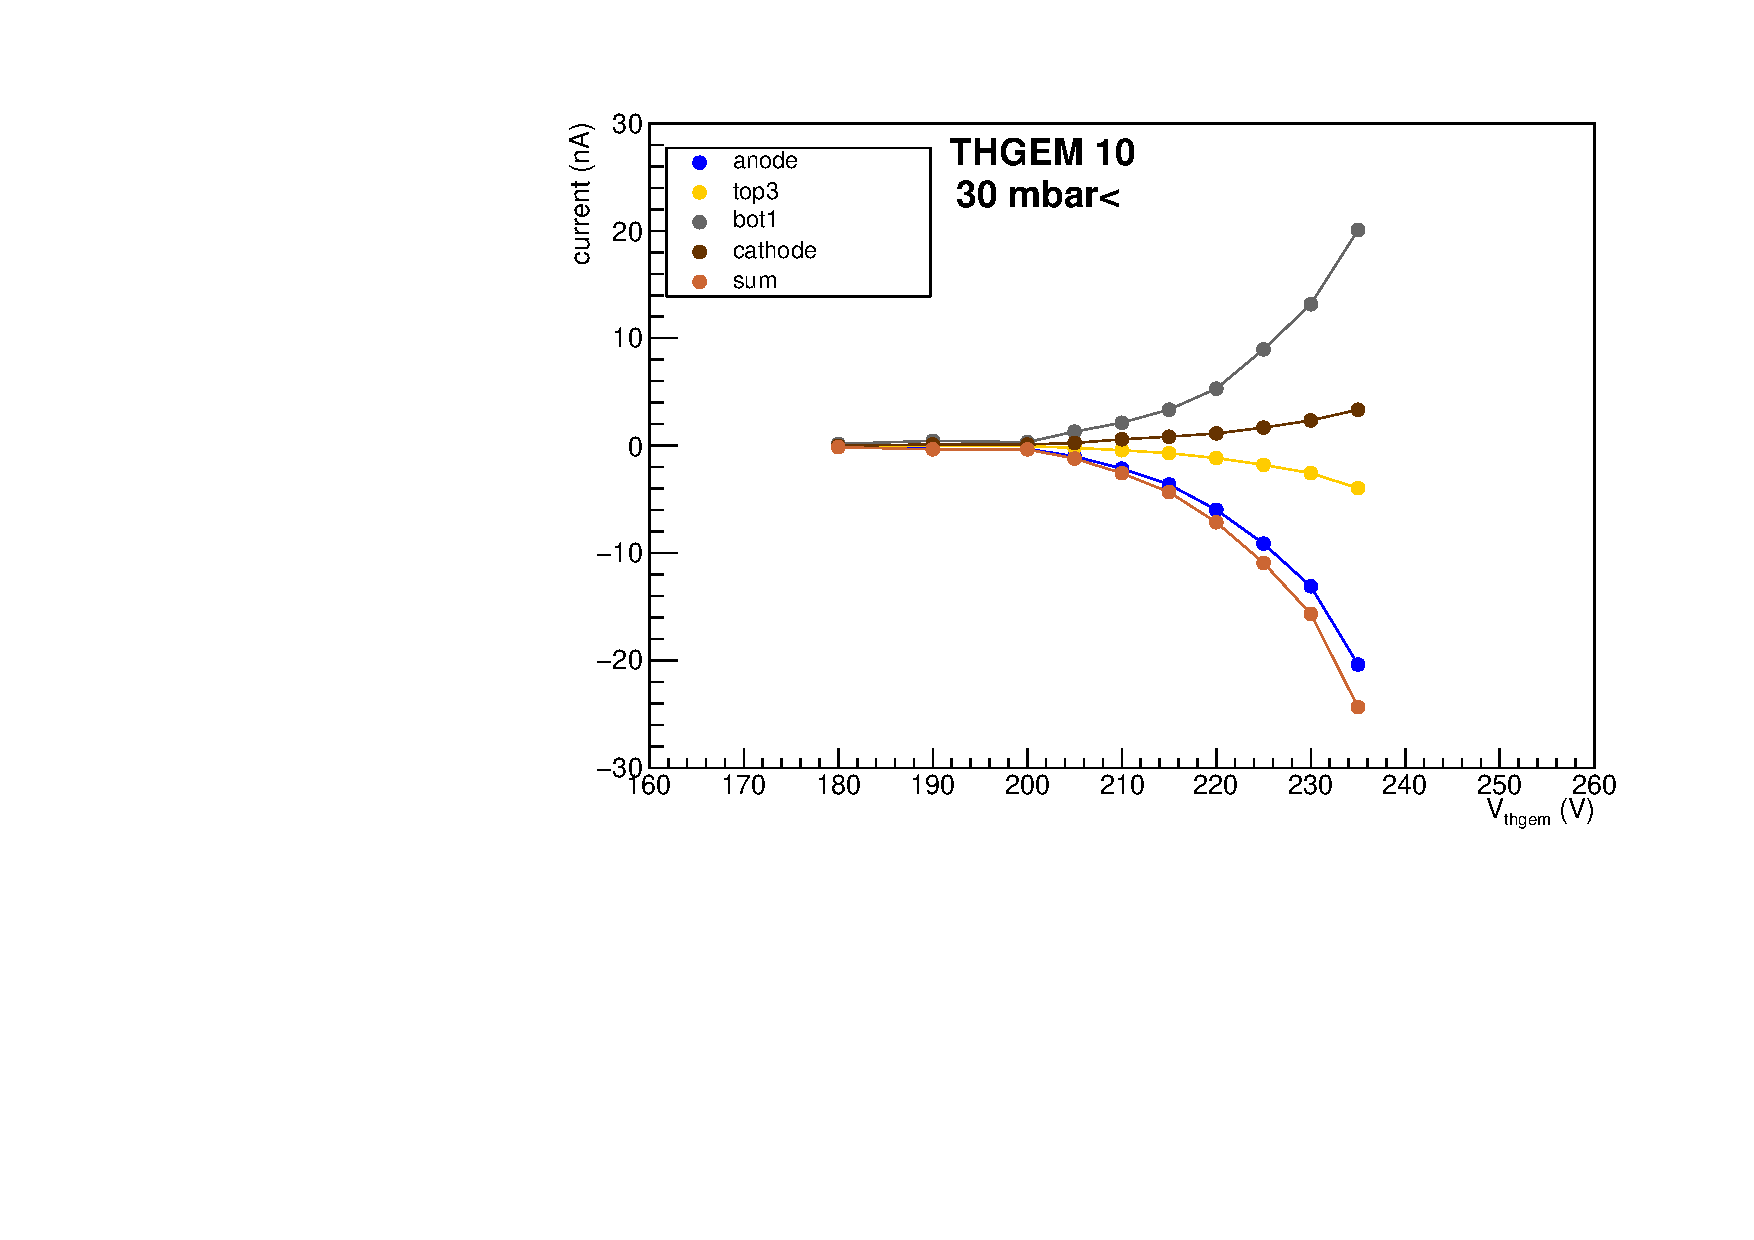
\includegraphics[width=0.9\textwidth]{Immagini/thgemScan_THGEM10_30mbar.pdf}
	\caption{Currents measured during the scan on the THGEM voltage at 30~mbar.}
	\label{fig:thgem_FULLTHGEM_30mbar}
\end{figure}






\subsubsection*{Scan on THGEM voltage  at 30 mbar}
To find the optimal value for the THGEM voltage until discharge, a scan on this parameter has been done.
The measured currents obtained for a pressure of 30~mbar and for \Vind~=~120~V and \Vdrift~=~1000~V are shown in Figure~\ref{fig:thgem_FULLTHGEM_30mbar}.

\Vthgem~=~180~V is the minimum voltage at which anode current is measurable.
At \Vthgem~=~230~V there was discharges, but we do not know if it came from THGEM.

The anode current has the typical exponential behaviour.



\subsubsection*{Scan on drift voltage  at 30 mbar}
To find the optimal value for the drift voltage until discharge, a scan on this parameter has been done.
The measured currents obtained for a pressure of 30~mbar and for \Vind~=~120~V and \Vthgem~=~220~V are shown in Figure~\ref{fig:drift_FULLTHGEM_30mbar}.

\begin{figure}
	\centering
	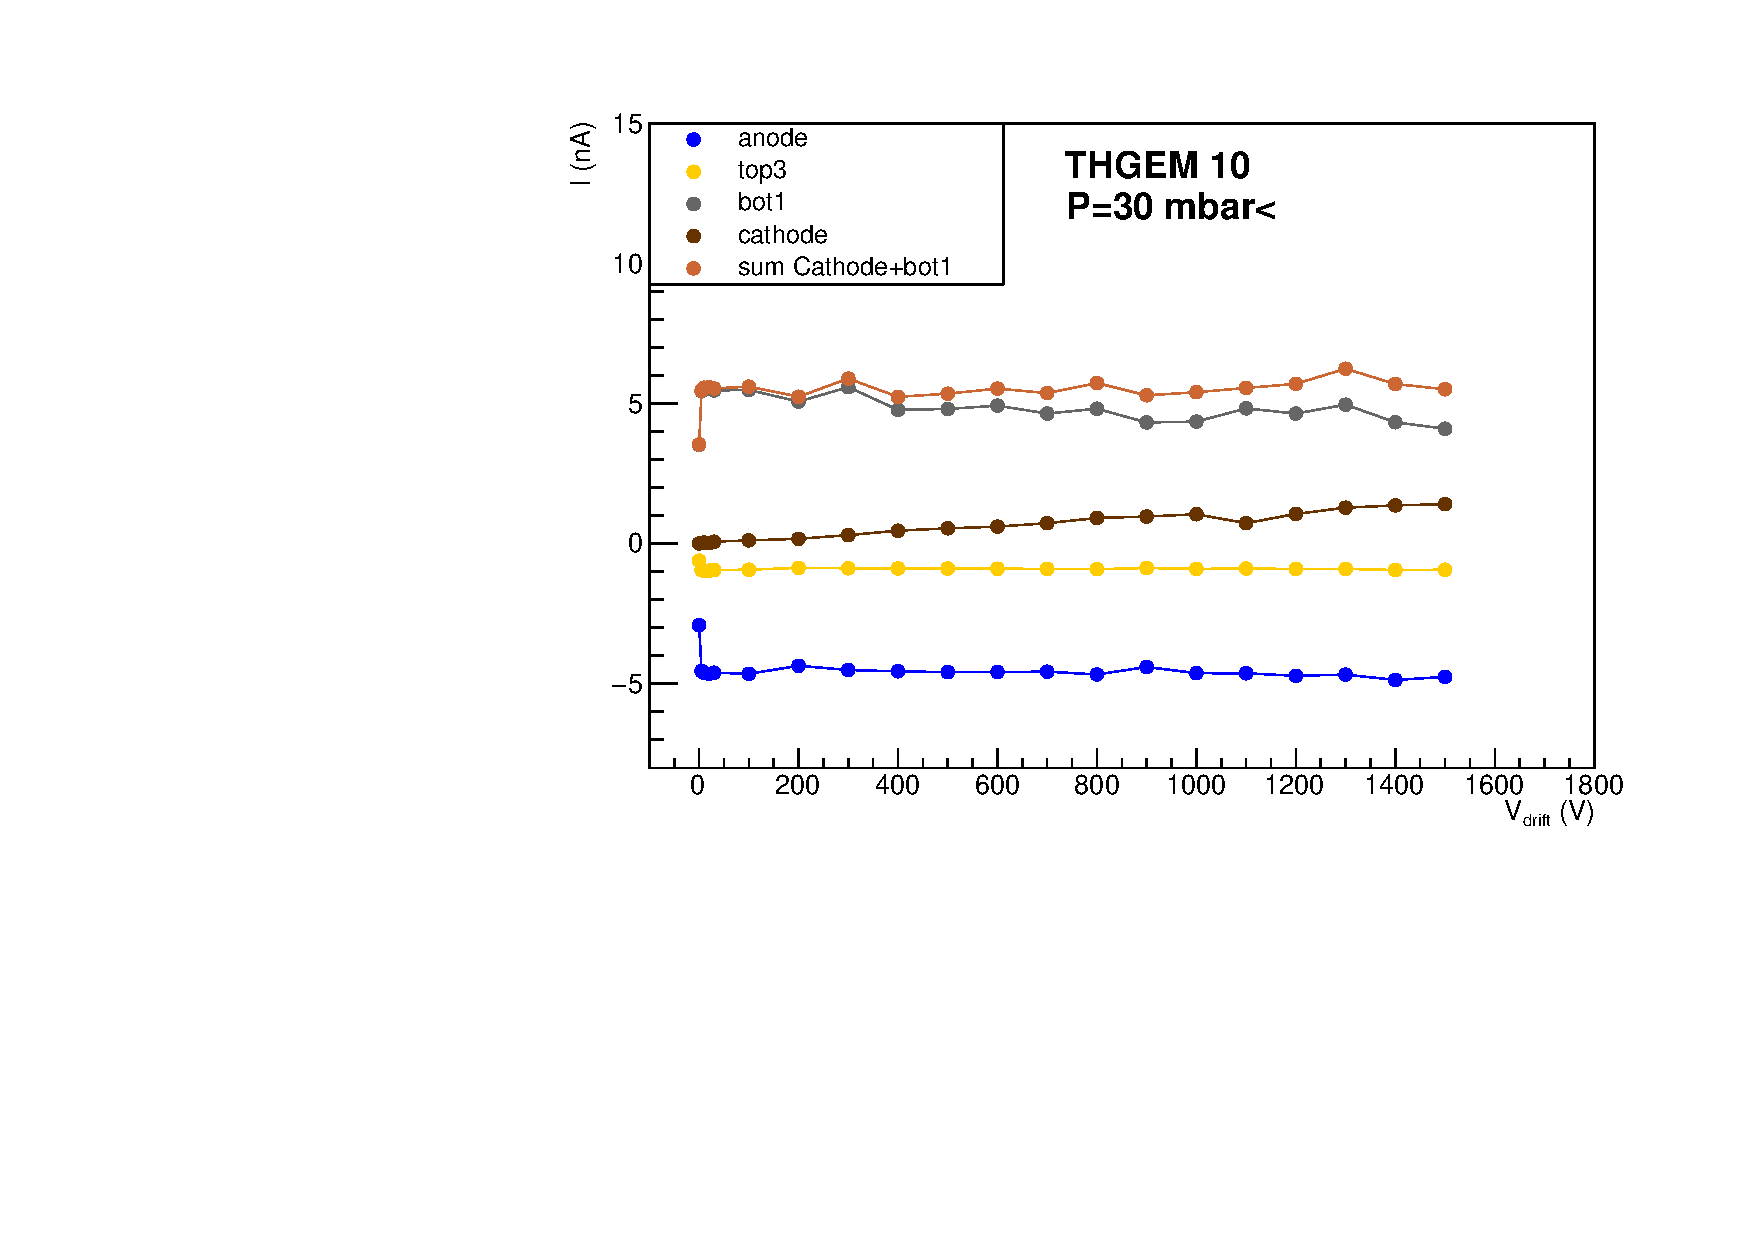
\includegraphics[width=0.9\textwidth]{Immagini/driftScan_THGEM10_30mbar.pdf}
	\caption{The currents measured during the scan on the drift voltage at 30~mbar.}
	\label{fig:drift_FULLTHGEM_30mbar}
\end{figure}

At \Vdrift~=~5~V the anodic current is saturated. 
This means that the magnitude of the electric field at \Vdrift~=~0~V is much lower than $\frac{5~V}{20~cm}= 250 mV/cm$ or the value measured by PICO is actually not zero.
At \Vdrift~=~1200~V ion backflow~(\ibf) is equal to 18.9\%, while at \Vdrift~=~1500~V \ibf~is equal to 24.7\%.
Dischages appeared at \Vdrift~=~1600~V.



\subsubsection*{Scan at 20 mbar}
The induction, THGEM and drift scan where repeated at 20~mbar and the currents curve show the same behaviour.

In \Vind~scan, \Vthgem~=~200~V and \Vdrift~=~1000~V and the plateau was in the range 90$\div$120~V.
The optimal value is 100~V.

In \Vthgem~scan, \Vind~=~100~V and \Vdrift~=~1000~V and the last measurable signal was at 150~V.
At 220~V there were discharges, so the optimal \Vthgem~value is 205~V.

During \Vdrift~scan, \Vind~=~100~V and \Vthgem~=~205~V and there were discharges at 1100~V.
At \Vdrift~=~700~V, the estimated value of \ibf is 13.2\%, whilst at \Vdrift~=~1000~V  \ibf is 17.3\%.


\subsubsection*{Scan at 10 mbar}
The induction, THGEM and drift scan where repeated at 10~mbar and the currents curve show the same behaviour.

In \Vind~scan, setting \Vthgem~=~180~V and \Vdrift~=~800~V, discharges appear at 60~V.
Setting \Vthgem~=~170~V and \Vdrift~=~800~V, there were discharges mainly in bot1 and cathode currents at 60~V.
So the chosen configuration is \Vthgem~=~170~V and \Vdrift~=~600~V. 
In this way, no discharges were visible.
The highest \Vind~value explored was 150~V.
Also for this pressure, a plateau was found in the range 60$\div$80~V.
The optimal value is 70~V.

In \Vthgem~scan, \Vind~=~70~V and \Vdrift~=~600~V and the last measurable signal was at 130~V.
At 210~V there were discharges, so the optimal \Vthgem~value is 190~V.

During \Vdrift~scan, \Vind~=~70~V and \Vthgem~=~190~V and there were discharges at 800~V.
At \Vdrift~=~450~V, the estimated value of \ibf is 10.9\%, whilst at \Vdrift~=~750~V  \ibf is 16.2\%.

\subsection{ROW THGEM}

\subsubsection*{Scan at 20 mbar}
The induction and THGEM scan where repeated at 20~mbar for ROW THGEM and the currents curve show the same behaviour as shown in Figure~\ref{fig:induction_ROWTHGEM_20mbar}.

In \Vind~scan, \Vthgem~=~220~V and \Vdrift~=~800~V but plateau is absent. Little discharges were visible up to \Vind~50V while big discharges in the range 60-110V affected bot1 and top3 currents. The optimal value is 50V.

\begin{figure}
	\centering
	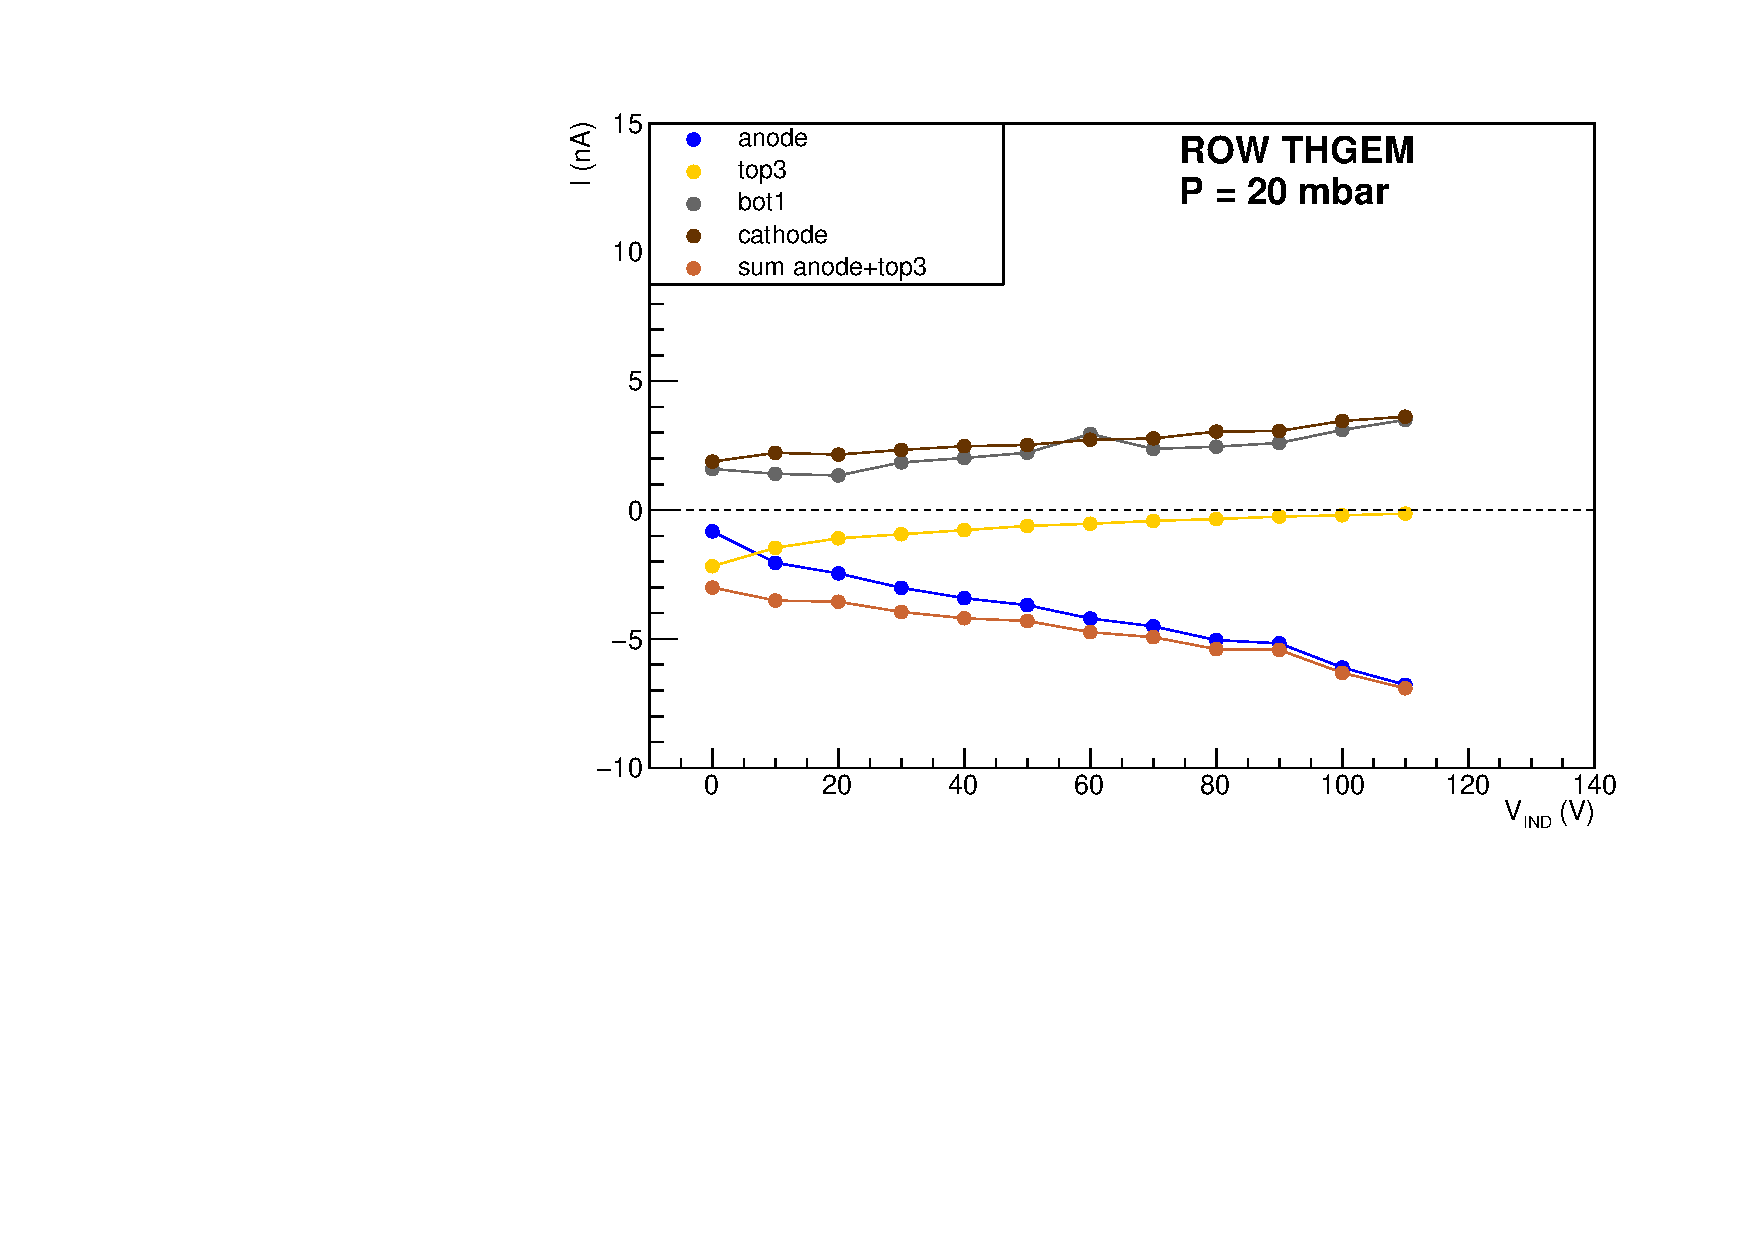
\includegraphics[width=0.9\textwidth]{Immagini/InductionScan_ROW_THGEM_20mbar.pdf}
	\caption{The currents measured during the scan on the induction voltage at 20~mbar.}
	\label{fig:induction_ROWTHGEM_20mbar}
\end{figure}

In \Vthgem~scan, \Vind~=~50~V and \Vdrift~=~800~V and the last measurable signal was at 180~V.
At 225~V there were big discharges, so the optimal \Vthgem~value is 210~V. We do not know if this value is the right one because no drift scan was made. 


%partiamo dalle full thgem:

%sulla parte di induzione: uno dei grafici con i quattro canali e la somma appropriata, incrocio fra corrente anodo e top3, regione di quasi plateau, poi la corrente aumenta, se avremo delle simulazione potremo corredare il discorso; obiettivo: cercare la regione di migliore funzionamento che dovrebbe essere quella del plateau



%sulla parte delle thgem: andamento esponenziale, si raggiunge il limite di scarica, non sappiamo se la scarica � nelle thgem



%sulla parte di drift: variare la corrente tra catodo e bottom1; a 0 volt abbiamo una misura: o lo strumento segna zero ma non � zerp 



descrizione delle varie pressioni: un grafico tenendo soltanto anodo a diverse pressioni, questo grafico non varia drammaticamente al variare della pressione; un altro grafico con l'induzione al variare della tensione delle thgem e/o del drift.



ion backflow: calcolare direttamente il valore in percentuale; unico grafico al variare delle pressioni; esso non dipende molto dall'induzione; esso dipende anche delle thgem (configurazione delle linee di forza); conclusione: 

fattore di moltiplicazione: inizialmente solo con le thgem piene;
poi thgem row e mostrare i tre grafici esemplari
induzione delle row thgem a 20 mbar � pi� bello;

%\subsection{ROW THGEM}

la drift � da discutere: la loro geometria � diversa: 5 fila isolate e proviamo a spiegare che a basse tensioni della drift, il campo elettrico delle thgem forma un imbuto pi� largo, se vdrift aumenta la regione da cui le thgem raccolgono carica diminuisce

dalle row thgem ci aspettiamo meno corrente perch� hanno meno buchi: invece di 143 file, ne hanno 5, quindi hanno il 3.5\% dei buchi rispetto a quelle piene. In prima approssimazione potremmo aspettarci che il valore della corrente scali allo stesso modo. 

ion backflow nelle row � sistematicamente pi� alto; vediamo se l'andamento � simile; al variare dell'induzione diminuzione dell'IBF; 

%ricordarsi di fare la misura del drift delle row a 20 mbar
%ATTENZIONE: altri test tenendo i campi elettrici fissi
%Misura ad alta pressione con full thgem, misura ad altre pressione con row thgem e rifare i test cercando di mantenere i campi elettrici costanti (possibilmente con il drift a tensioni basse)



\section{Conclusioni}




\end{document}
